
\section{Crear un issue desde la página web}

Para crear un issue desde la página web de GitHub, primero me uní a un repositorio colaborativo. Una vez en dentro del repositorio, debemos de dirigirnos a la pesaña de issues y luego damos clic en nuevooo issue "New issue". Ahora, agregamos una descripción, un título al issue, podemos agregar una etiqueta (aparecen en la parte de la derecha y dice "label") dependiendo para que caso.

\begin{figure}[H]
    \centering
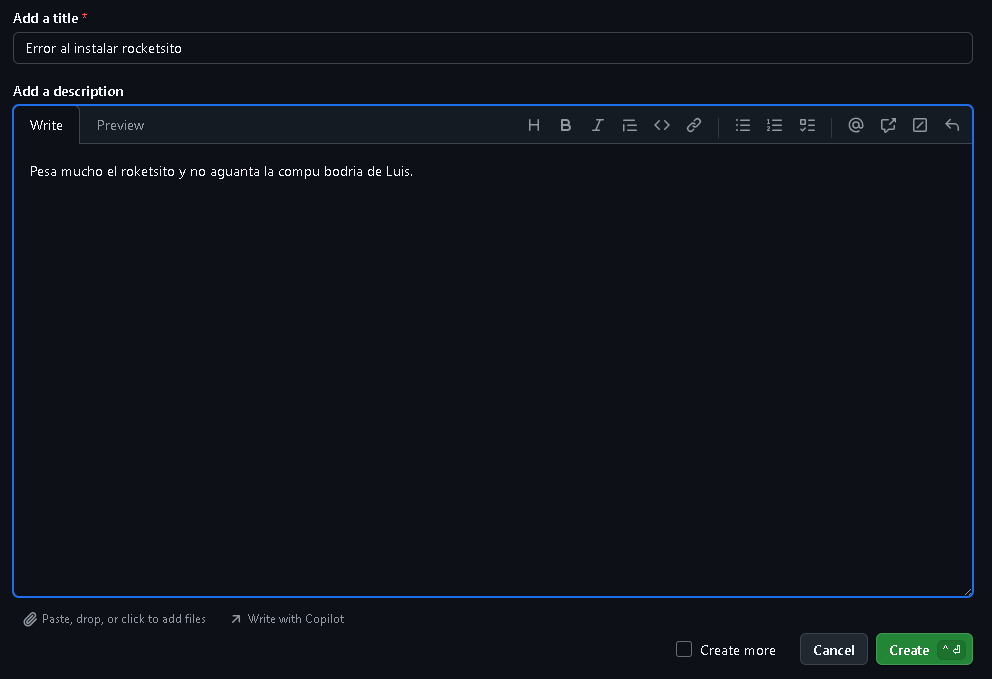
\includegraphics[width=1\textwidth]{imagenes/img/issue1.png}
    \caption{Creación de un issue desde la página web}
    \label{fig:D1}
\end{figure}

\begin{figure}[H]
    \centering
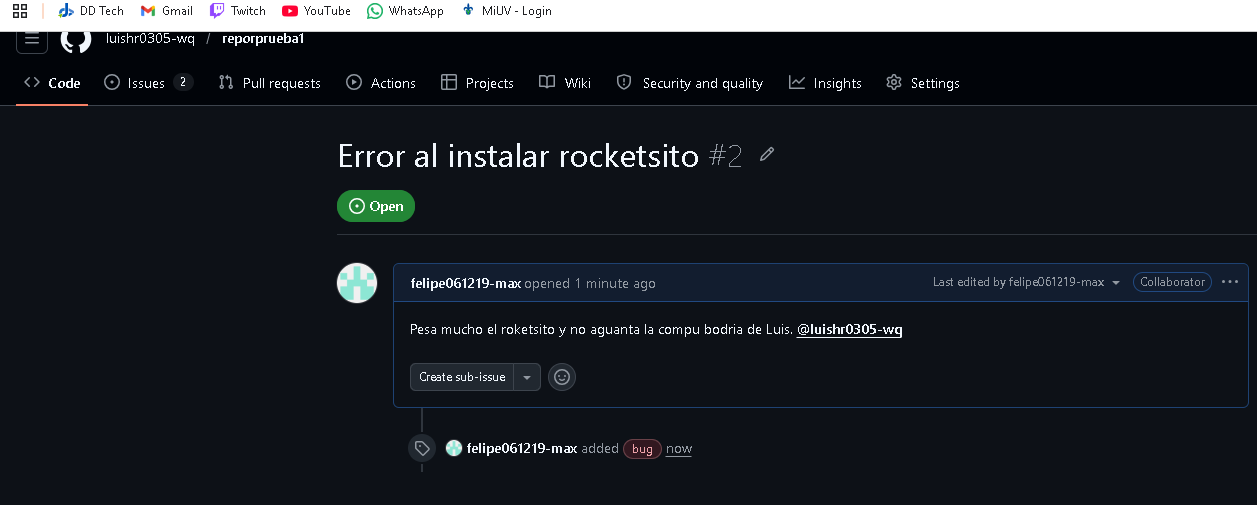
\includegraphics[width=1\textwidth]{imagenes/img/issue2.png}
    \caption{Agregar etiquetas}
    \label{fig:D2}
\end{figure}

Aquí ya podemos visualizar los issues abiertos y cerrados del repositorio, así como la etiqueta del issue y el responsable.

\begin{figure}[H]
    \centering
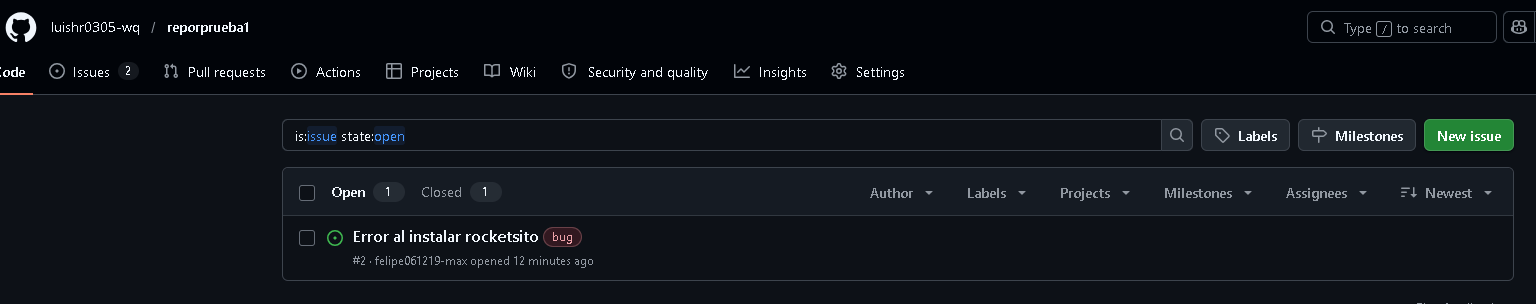
\includegraphics[width=1\textwidth]{imagenes/img/issue3.png}
    \caption{Visualización del issue en el repositorio}
    \label{fig:D3}
\end{figure}

\begin{figure}[H]
    \centering
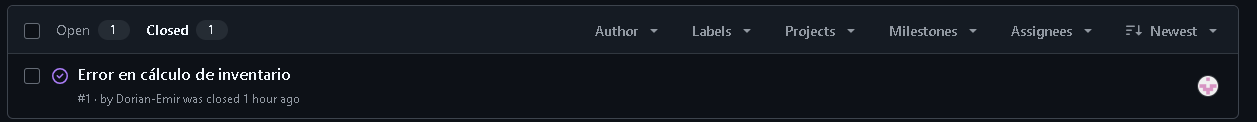
\includegraphics[width=1\textwidth]{imagenes/img/issue_c.png}
    \caption{Visualización del issue en el repositorio}
    \label{fig:D4}
\end{figure}